\documentclass{standalone} 
\PassOptionsToPackage{usenames,dvipsnames,svgnames}{xcolor}  
\usepackage{tikz}
\usetikzlibrary{arrows,positioning,automata}

\begin{document}
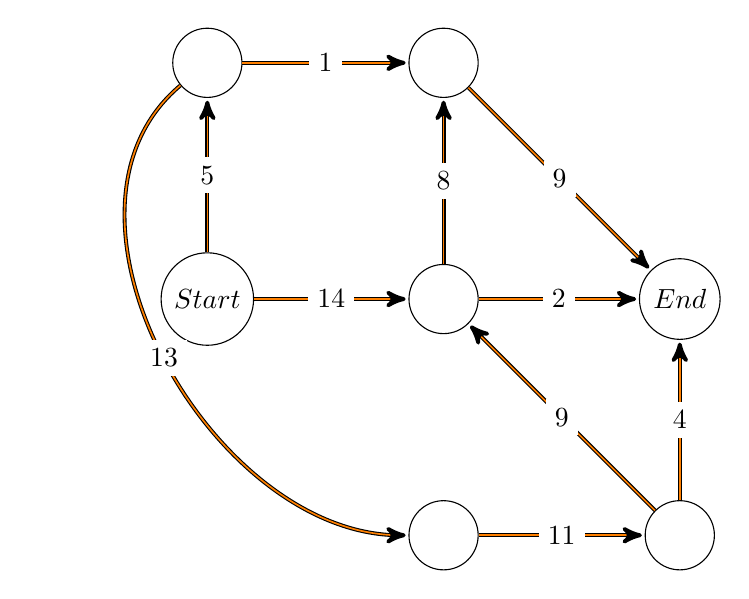
\begin{tikzpicture}[>=stealth',shorten >=1pt,node distance=3cm,on grid,initial/.style    ={}]
  \node[state]          (P)                        {$Start$};
  \node[state]          (B) [above       =of P]    {};
  \node[state]          (D) [      right =of B]    {};
  \node[state]          (C) [below       =of D]    {};
  \node[state]          (L) [      right =of C]    {$End$};
  \node[state]          (X) [below       =of C]    {};
  \node[state]          (Y) [below       =of L]    {};
\tikzset{mystyle/.style={->,double=orange}} 
\tikzset{every node/.style={fill=white}} 
\tikzset{mystyle/.style={->,double=orange}}   
\path (P)     edge [mystyle]   node   {$5$} (B)
      (B)     edge [mystyle]   node   {$1$} (D)
      (B)     edge [mystyle,in=180,out=220]   node   {$13$}(X)
      (P)     edge [mystyle]   node   {$14$}(C)
      (C)     edge [mystyle]   node   {$8$} (D)
      (D)     edge [mystyle]   node   {$9$} (L)
      (C)     edge [mystyle]   node   {$2$} (L)
      (X)     edge [mystyle]   node   {$11$}(Y)
      (Y)     edge [mystyle]   node   {$4$} (L)
      (Y)     edge [mystyle]   node   {$9$} (C);
\end{tikzpicture}
\end{document}